\chapter{Background Ensemble}\label{sec:backgroundEnsamble}

This note discusses a strategy for estimating the spurious signal. This analysis uses a background estimation defined with a fit to data. This note describes how the spurious signal is estimated for this data-driven background.
This procedure is described in detail, however the essential idea is as follows: the spurious signal is measured from an ensemble of \emph{plausible} background shapes that are informed by systematic uncertainties.

\subsection*{Challenge}

We define our expected background using a PDF, \func, fit to a dataset \template with dimension \ddata. The full analysis procedure of fitting the dataset and obtaining a background estimate is described by the function \eeNbkg, with a range of dimension \dbkg and domain of dimension \ddata. The output of \eeNbkg is the expected background, given the provided dataset \template. The remainder of this procedure is agnostic with regard to the particular definition of \eeNbkg. In the case of the Non-Resonant search, \eeNbkg is the fitting and extrapolation procedure, where \ddata is the number of bins in the Control Region, and \dbkg is the single bin of the Signal Region.

A main uncertainty on \eeNbkg is the spurious signal \spur.
We define \spur as the number of signal events measured via \eeNbkg, given \template is a background-only Asimov dataset.
As with \eeNbkg, we consider $\spur(\template)$ to be a function of a potential background shape \template.
To discuss this, let's define the potential background-only distributions on which \eeNbkg can operate:
\begin{enumerate}
    \item \mc, the nominal simulated background, with enough events to mitigate statistical fluctuations.
    \item \syst, a set of simulated systematic variations on the nominal background.
    \item \data, the recorded dataset which will be used for the final background estimation. We consider this recorded data to be randomly sampled from a ``true'' PDF, \truth.
    \item \truthdata, the Asimov dataset generated by \truth. In practice, this is not known.
\end{enumerate}
For illustration purposes, examples of these are shown in figure \ref{fig:datasets}.

\begin{figure}[!htpb]
\centering
\subfloat[][]{{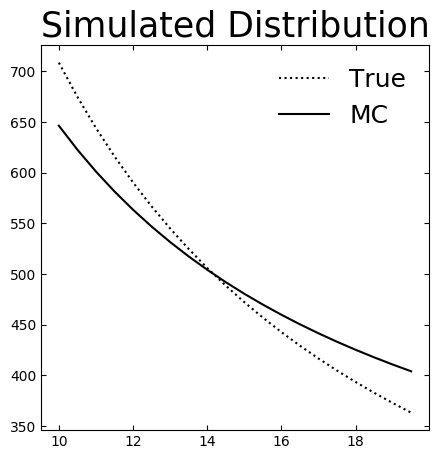
\includegraphics[width=0.3\textwidth]{figures/backgroundEnsamble/mc.png}}}
\subfloat[][]{{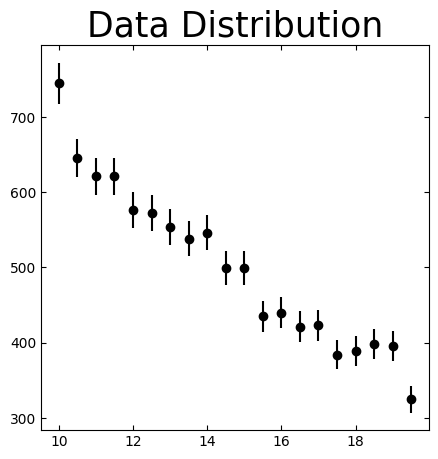
\includegraphics[width=0.3\textwidth]{figures/backgroundEnsamble/data.png}}}
\subfloat[][]{{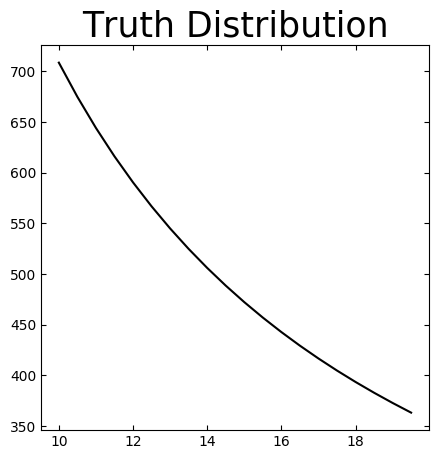
\includegraphics[width=0.3\textwidth]{figures/backgroundEnsamble/asimov.png}}}
\caption{Examples of \mc (a), \data (b), and \truthdata (c). \mc is shown to diverge from the true underlying distribution that has generated the data.}
\label{fig:datasets}
\end{figure}


It is trivial to measure the \spur that corresponds to \mc, denoted $\spur(\mc)$. This is usually done by computing \nbkgmc, and measuring the number of signal events spuriously recovered from the procedure.
However if we want to measure $\spur(\data)$ and use it in the analysis, we are faced with three main concerns:
\begin{enumerate}
    \item \data may not be a background-only distribution, and we certainly do not want to assume that it is before making a measurement.
    \item Due to limited statistics, \data is not an Asimov dataset, and therefore \nbkgdata will be influenced by the statistical fluctuations of the recorded data.
    \item The most fundamental issue is that the \spur measured from \nbkgdata is essentially our signal measurement.
\end{enumerate}

If we want to use \nbkgdata for the expected background, we need an alternative way to estimate \spur.
We cannot use \spur estimated from \nbkgdata for the reasons listed above.
We prefer not to simply use \spur estimated from \nbkgmc, since this makes the assumption that \mc was sampled from a PDF matching \truth.
Instead, we would like to use \spur measured from \nbkgtruth.
Since we do not know \truthdata, we use the procedure described here to obtain our best estimate of \truthdata given our available prior knowledge.

\subsection*{Approach}

The exact form of \truthdata is not known. While our best theoretical estimate of the exact shape of \truthdata may be \mc, this does not encompass our all of our information. Since \truthdata is a \dbkg dimensional vector, we know that $\truthdata\in\realsBkg$. Likewise, $\mc\in\realsBkg$. Going further, we have a strong suspicion that \truthdata is ``close'' to \mc within \realsBkg. One could consider the systematic uncertainties \syst as a description of how close \truthdata is to \mc. Instead, we would like to use \syst to define a PDF \map corresponding to the estimated likelihood of finding \truthdata to be at a particular point in \realsBkg. In the future, we would like to rework this Bayesian reasoning to a more frequentist one.

For each systematic variation \syst, we define a nuisance parameter $\np\in\eeReal$. For simplicity, consider that \np are defined such that have $1\sigma$ confidence that the value of \npmeasured measured on \truthdata is $\in[-1,1]$, and $\np=0$ corresponds to \mc. This allows us to define \emph{Standard Gaussian} priors for each systematic, \npprob. (If the upward and downward variations are measured separately, \npprob can still be a Standard Gaussian and the impact of $\np>0$ can be treated differently than $\np<0$.) Taken together, \np define a vector $\nps\in\realsSyst$. This leads to a simplification wherein we now consider the dimensionally smaller $\nps\in\realsSyst$ instead of the full $\template\in\realsBkg$, as long as $\dsyst<\dbkg$. The measured shapes of the systematics, \systs, are used to map choice of \nps onto a full background shape: \mapThetaToBkg. An example of this map is shown later in Equation \ref{map}.

Each choice of $\nps\in\realsSyst$ has a prior expected probability of:
\begin{equation}\label{thetaProb}
p(\nps) = \prod_{i=0}^{\dsyst}\npprob.
\end{equation}

We should also keep in mind that we are essentially assigning a prior probability to each choice of $\template\in\realsBkg$:
\begin{equation}\label{dataProb}
\begin{split}
% p(\template) =& \sum_{\{j|g(\nps_j)=\template\}} p(\nps_j) \\
p(\template) =& \oint_{\realsSyst} p(\nps)~\delta(g(\nps_j)-\template)~d\nps \\
\end{split}
\end{equation}
This $p(\template)$ is zero for many non-physical choices of \template, since these cannot be represented by a choice of nuisance parameters.

Now we can return to the goal of approximating $\spur(\truthdata)$. As a substitute, we propose to calculate $\spur(\template)$ for every $\template\in\realsBkg$. These are then weighted by the corresponding probability $p(\template)$:
\begin{equation}\label{weighted}
\deltaD(\template) = p(\template) \times \spur(\template).
\end{equation}
The resulting distribution of \deltaD represents the spurious signal for every possible background shape \template, weighted by the likelihood that each the $\template=\truthdata$.
We consider the mean of this distribution, \meanD, to be our best estimate of $\spur(\truthdata)$, and the width of this distribution, \stdD, to be our uncertainty on that estimate.

Every choice of \nps maps onto a \template. Therefore, we can measure the spurious signal as $\spur(\nps)=\spur(g(\nps))$, and define a quantity analogous to Equation \ref{weighted}:
\begin{equation}\label{weighted2}
\begin{split}
\deltaTheta(\nps) =& p(\nps) \times \spur(\nps).
\end{split}
\end{equation}

The value of \meanD is measured over the volume of potential values of \template. The denominator of the mean is $\oint_{\realsBkg} p(\template)=1$. A couple of substitutions show that we can calculate \meanTheta instead of \meanD.
\begin{equation}\label{meansEqual}
\begin{split}
\mathrm{\meanD} =& \oint_{\realsBkg} p(\template)~\spur(\template) ~d\template  \\
           % =& \oint_{\realsBkg} \left(\sum_{\{j|g(\nps_j)=\template\}} p(\nps_j)\times \spur(\template)\right) d\template / \oint_\realsBkg d\template \\
           =& \oint_{\realsBkg} \left(\oint_{\realsSyst} p(\nps)~\delta(g(\nps)-\template)~d\nps\right)~\spur(\template) ~d\template  \\
           =& \oint_{\realsSyst} p(\nps)~\spur(\nps)~d\nps  \\
\mathrm{\meanD} =& \mathrm{\meanTheta} \\
\end{split}
\end{equation}

The value of \stdD can be replaced with \stdTheta using similar substitutions from Equation \ref{meansEqual}:
\begin{equation}\label{stdevsEqual}
\begin{split}
\stdD =& \sqrt{\meanDSquared-(\meanD)^2} \\
             =& \sqrt{\meanThetaSquared-(\meanTheta)^2} \\
\stdD =& \mathrm{\stdTheta} \\
\end{split}
\end{equation}

Based on Equations \ref{meansEqual} and \ref{stdevsEqual}, we will measure \meanTheta and \stdTheta as an estimate of $\spur(\truthdata)$.

\subsection*{Implementation}

Our goal is to compute \meanTheta and \stdTheta. Since \deltaTheta is weighted by a probability p(\nps), we take the straight forward approach of obtaining the distribution of \deltaTheta via a Monte-Carlo random sampling of the possible values of $\nps\in\realsSyst$. We choose values for \nps selected randomly based on the priors \npprob for each nuisance parameter \np. Each choice of \nps corresponds to a ``toy'' dataset \template, where the probability of being selected corresponds to $p(\nps)$.

For each toy $\nps_j$, we calculate $\spur(\nps_j)$. The distribution of $\spur(\nps_j)$ toy measurements, in the limit of many toys, approaches the distribution of \deltaTheta. The enumerated procedure to build a distribution of $\spur(\nps_j)$ is as follows:
\begin{enumerate}
    \item For each \np a random value is sampled from the PDF \npprob. This selects a point $\nps_j$.
    \item Using the information from \mc and \systs, $\nps_j$ determines a toy background shape $\template_j$. For example,
            \begin{equation}\label{map}
               \template_j = \mc + \sum_{i=0}^{\dsyst} (\syst-\mc)\times(\nps_j)_i.
            \end{equation}
    \item Compute $\spur(\template_j)$, the spurious signal measured on the toy dataset $\template_j$.
\end{enumerate}

Next, we measure the mean and standard deviation of the toy measurements, as an approximation of \meanTheta and \stdTheta respectively. We then use these to approximate $\spur(\truthdata)$ with a corresponding uncertainty. This allows us to estimate our background from the data using \nbkgdata, and with this use a \spur that we believe corresponds to the underlying PDF that generated \data.

\subsection*{Caveats}

The following is a brief discussion about some of the complexities that arise when implementing this procedure.

\subsubsection*{The $1\sigma$ approximation}

In this procedure, we represent our systematic uncertainties as prior PDFs.
Ideally, these PDFs would be measured for many different confidence intervals.
In practice, these are often measured as the $\pm 1\sigma$ intervals in which the systematic variation is expected.
We then make the assumption that the $\pm n\sigma$ interval is n-times the size of the $\pm 1\sigma$ interval.
In doing this, we are making the assumption that the shape of the prior PDF is Gaussian.
In some cases this assumption may be unreasonable; for example if the $-3\sigma$ $p_T$ variation is negative.

\subsubsection*{Asymmetric systematics}

Equation \ref{map} shows one form of \thetaToBkg, a map from \nps to a background shape. In practice, a more nuanced version should be used because systematics are measured in different ways.
A subset of systematics with indices $\mathbb{A}\in\{1,2,...,\dsyst\}$ may be measured separately to produce upper, \systUp, and lower, \systDn, uncertainty bands. We still consider these to be described by one nuisance parameter \np with a Standard Gaussian prior:
\begin{equation*}
   p(\np) = \npprob.
\end{equation*}
To handle the asymmetry of \systUp and \systDn, we modify the impact of \np on each toy ($j$) template $\template_j$. We are sculpting the impact of \np on the toy shape in order to preserve the symmetrical Gaussian prior. Equation \ref{map} is expanded to treat symmetric and asymmetric systematics separately:
\begin{equation}
\begin{split}
   \template_j =& \mc + \sum_{i\in~\mathbb{B}}(\systUp-\mc)\times(\nps_j)_i + \sum_{i\in~\mathbb{C}}(\systDn-\mc)\times(\nps_j)_i + \sum_{i\in~\mathbb{D}}(\syst-\mc)\times(\nps_j)_i \\
\end{split}
\end{equation}
\vspace{-1em}
\begin{equation*}
\begin{split}
   \mathbb{B}           =& \{i\in \mathbb{A}|(\nps_j)_i>0\} \\
   \mathbb{C}           =& \{i\in \mathbb{A}|(\nps_j)_i<0\} \\
   \mathbb{D}           =& \{i\notin \mathbb{A}\} \\
\end{split}.
\end{equation*}
Here, symmetric systematics are treated as before, while asymmetric systematics use the uncertainty band corresponding to whether $(\nps_j)_i$ is positive or negative.
This is straightforwardly implemented with conditionals when building the toy template $\template_j$.

\subsubsection*{Envelope uncertainties}

In the Non-Resonant search, the many dominant systematics (PDC\_Choice, Bad-Muon-Veto, etc.) are measured as \emph{envelopes}. These are statements that \truthdata falls within a particular range. This formulation of systematic uncertainty does not lend itself easily to a simple description of a prior on a corresponding nuisance parameter. One choice of the prior $G'$ be a flat step function:
\begin{equation*}
    G'(\np)=
\begin{cases}
    1/2             & \text{if }|\np|\le1 \\
    0               & \text{otherwise}
\end{cases}.
\end{equation*}
This choice does not reflect our belief that the nominal \mc is more likely than the extreme bounds of the envelope. Another choice of the prior would be a Gaussian, such as is appropriate for Gaussian distributed nuisance parameters. This leads to an enlarged impact from the envelope systematics, since now large deviations corresponding to $\np>1$ are allowed. This is in conflict with the statement of the envelope, that such shapes are excluded (though to what level is not clear). The third option is a compromise is a Gaussian prior restricted to the confines of the envelope:
\begin{equation*}
    G'(\np)=
\begin{cases}
    \frac{G(\np)}{\text{erf}(\sqrt{0.5})}            & \text{if }|\np|\le1 \\
    0                                                & \text{otherwise}
\end{cases}.
\end{equation*}
While this choice of PDF is not ideal (as mentioned above, we would prefer to measure the PDF at a number of intervals when assessing the impact of the systematic), it is a compromise between our physical intuitions and the requirement that the allowed variation fall within the measured envelope.

